\begin{frame}{Implementation: Knox}
\begin{columns}
  \column{0.48\linewidth}
  \centering
  \begin{outline}
  \1 Knox, monolithic verification
  \2 Source on \href{https://github.com/anishathalye/knox}{Github}
  \2 Hybrid Symbolic Execution \cite{Torlak2014lightweight}
  \1 Targets Rosette \cite{Torlak2013Growing}
  \2 Solver-aided programming language
  \1 Generate SMT Constraints
  \2 Solve with Z3 \cite{De2008Z3}
  \end{outline}

  \column{0.48\linewidth}
  \centering
  \begin{center}
  
\includegraphics[width=3cm]{racket_logo.png}
  
\includegraphics[width=1cm]{z3_logo.jpg}

  \vspace{0.5cm}

  
\includegraphics[width=5cm]{rosette_logo.png}

  \vspace{0.5cm}

  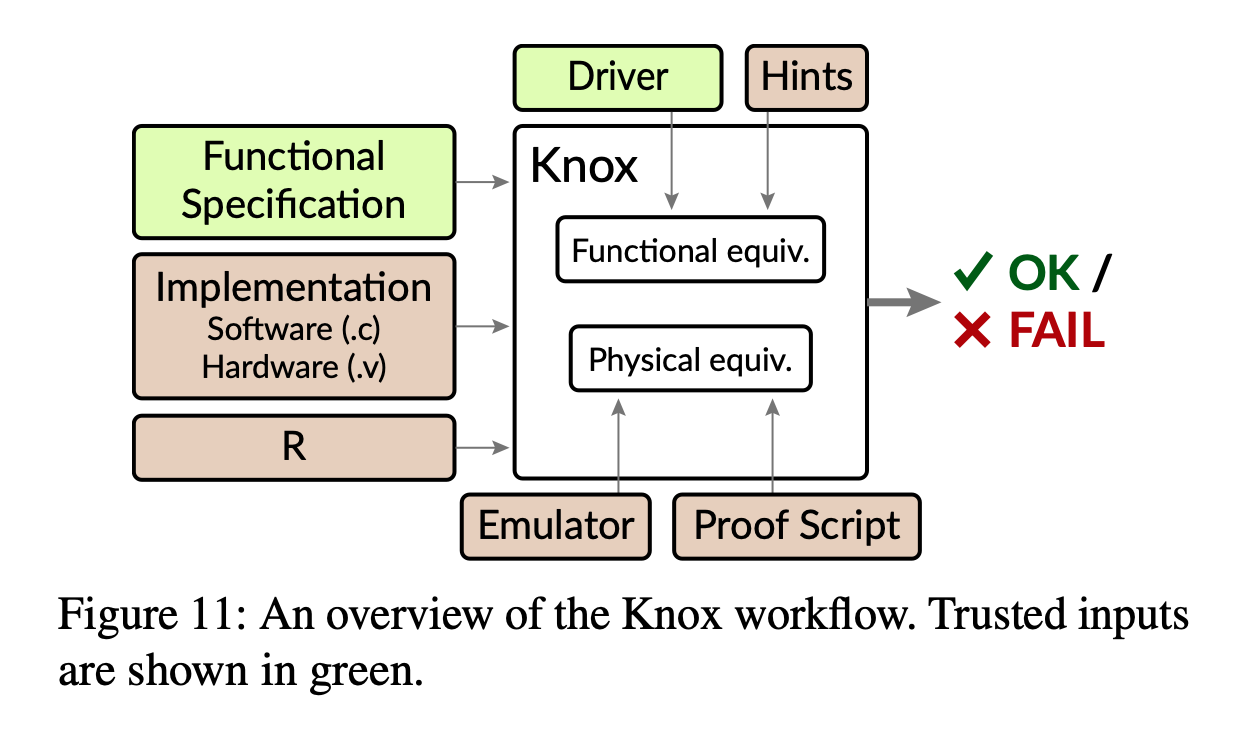
\includegraphics[width=5cm]{fig_11.png}

  \end{center}
\end{columns}
\end{frame}

\begin{frame}{Symbolic Execution}
  \begin{columns}
    \column{0.58\linewidth}
\begin{outline}
  \1 Functional Equivalence - \lstinline{yeild}
  \2 How to handle Nondeterminism?
  \2 Find closure of circuit states 
  \2 Fork on elements of set
  \2 Exponential growth!
  \2 \textit{merge} hints shrink space
  \1 Physical Equivalence - input size
  \2 Arbitrary sequence of wire inputs
  \2 Intractable to write circuit invariant
  \2 \textit{Guided symbolic model checking}
  \1 Knox allows variety of hints
\end{outline}
    \column{0.38\linewidth}
  \centering
  \begin{center}
  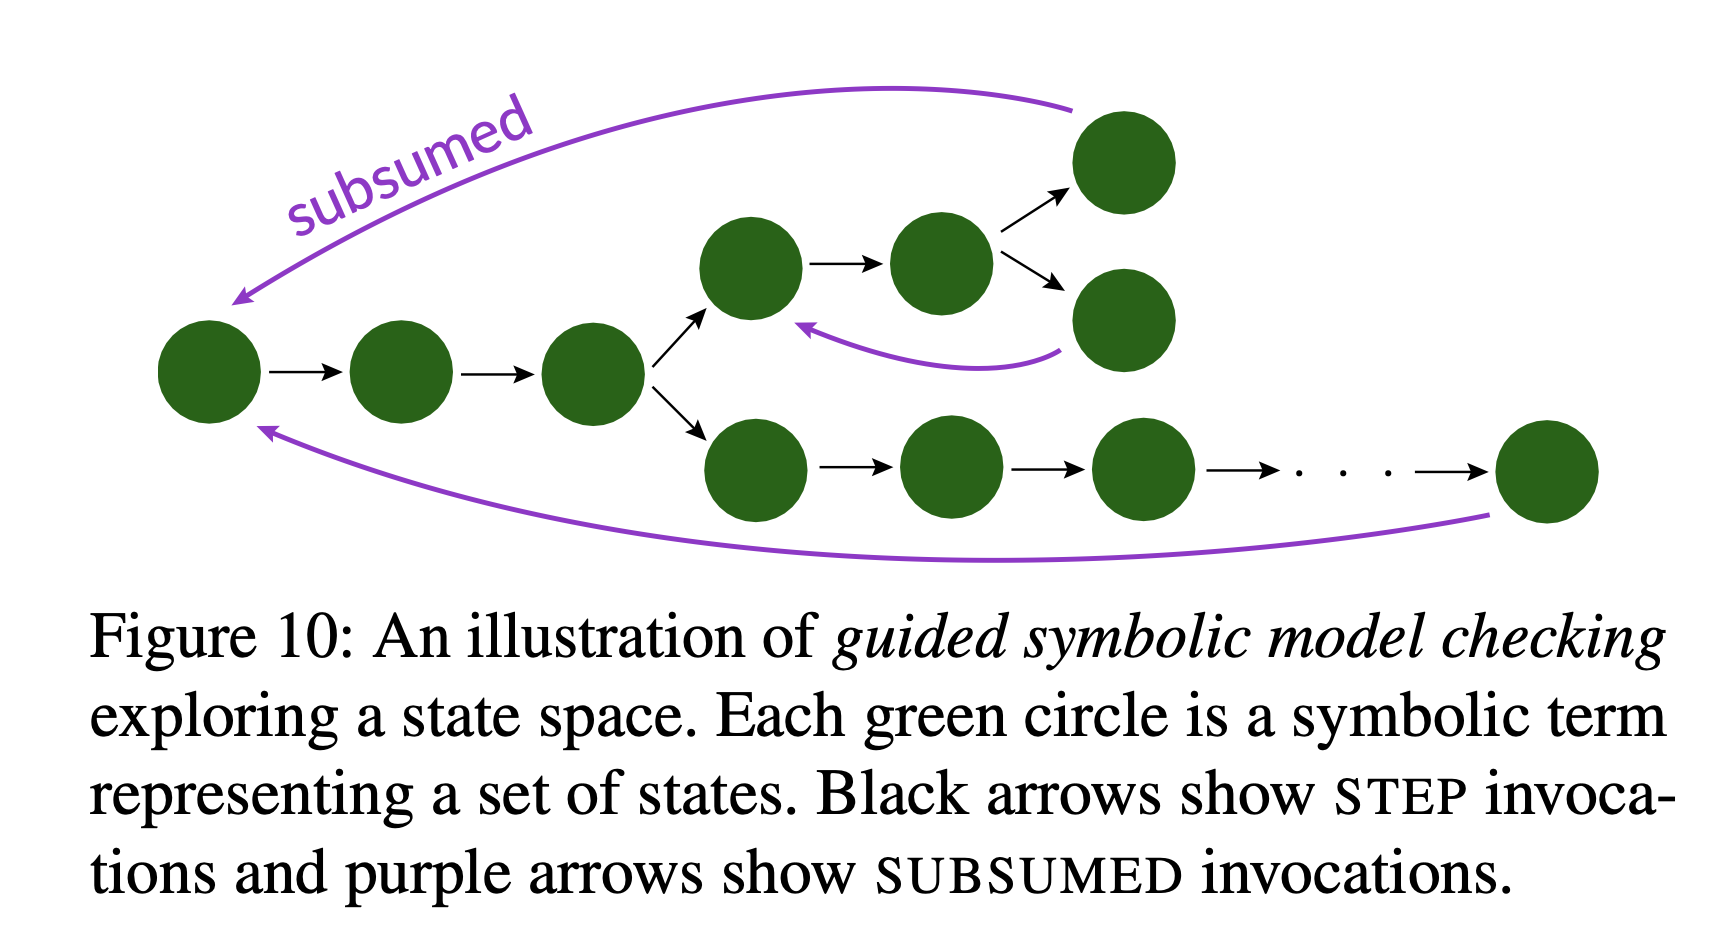
\includegraphics[width=4.5cm]{fig_10.png}
\end{center}
  \end{columns}
\end{frame}
